\documentclass{article}
\usepackage{blindtext}
\usepackage[utf8]{inputenc}
\usepackage{amsmath,bm}
\usepackage{amstext}
\usepackage{amsfonts}
\usepackage{amsmath}
\usepackage{multirow}
\usepackage{enumerate}
\usepackage{xeCJK}
\setCJKmainfont{STKaiti}
\usepackage{algorithm}
\usepackage{algorithmic}
\renewcommand{\algorithmicrequire}{ \textbf{输入:}} %Use Input in the format of Algorithm
\renewcommand{\algorithmicensure}{ \textbf{输出:}} %UseOutput in the format of Algorithm
\usepackage{graphicx}
\usepackage{booktabs}
\usepackage{listings}
\lstset{
	columns=fixed,       
	numbers=left,                                        % 在左侧显示行号
	numberstyle=\tiny\color{gray},                       % 设定行号格式
	frame=none,                                          % 不显示背景边框
	keywordstyle=\color[RGB]{40,40,255},                 % 设定关键字颜色
	numberstyle=\footnotesize\color{darkgray},           
	commentstyle=\it\color[RGB]{0,96,96},                % 设置代码注释的格式
	stringstyle=\rmfamily\slshape\color[RGB]{128,0,0},   % 设置字符串格式
	showstringspaces=false,                              % 不显示字符串中的空格
	language=python,                                        % 设置语言
}

\title{Neural Network and Applications\\Homework 4}
\author{陈轶洲 MF20330010}
\begin{document}
	\maketitle
	\numberwithin{equation}{section}
	
\section{}
首先设计类DBMOON()生成双月数据:
\begin{figure}[H]
	\centering
	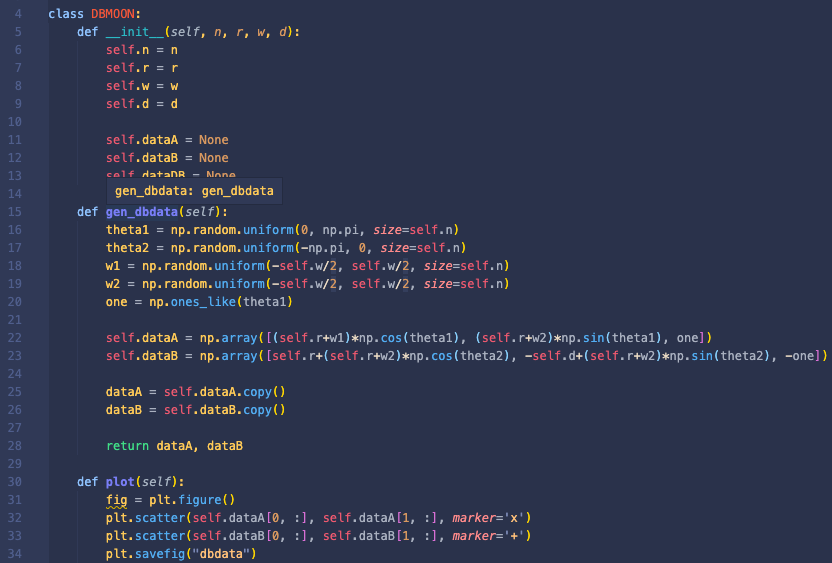
\includegraphics[scale=0.5]{dbmoon.png}
	\caption{类DBMOON}
\end{figure}

利用该类中的gen\_dbdata(1000,10,6,-2)生成2000个样本点,如下图所示:
\begin{figure}[H]
	\centering
	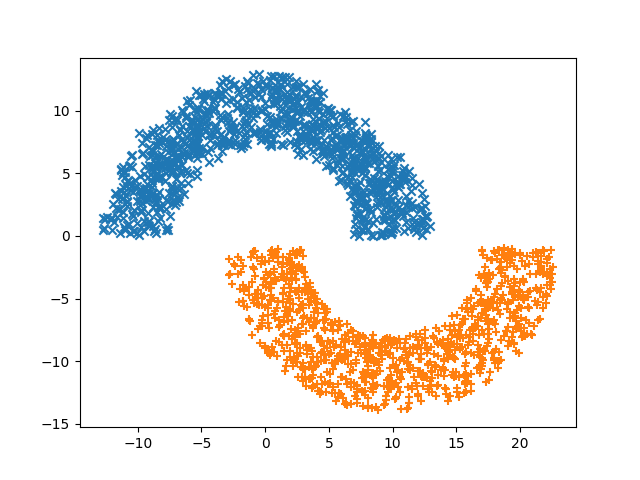
\includegraphics[scale=0.6]{code/dbdata.png}
	\caption{样本点}
\end{figure}

设计类SLP实现单层感知器的功能:
\begin{figure}[H]
	\centering
	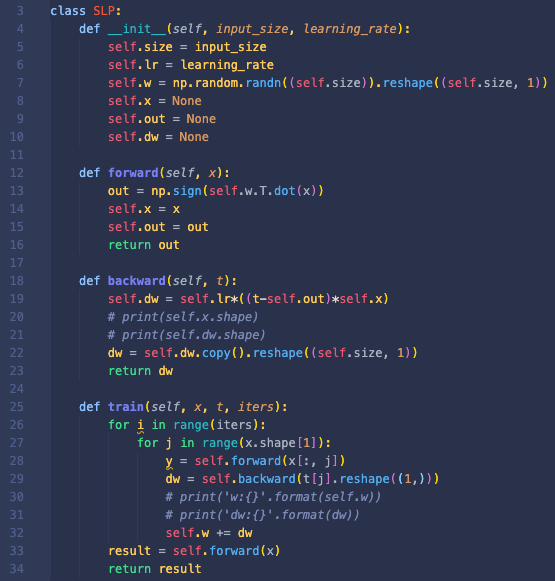
\includegraphics[scale=0.4]{slp.png}
	\caption{单层感知器}
\end{figure}

利用此单层感知器进行数据分类的学习,完成后画出决策边界:
\begin{figure}[H]
	\centering
	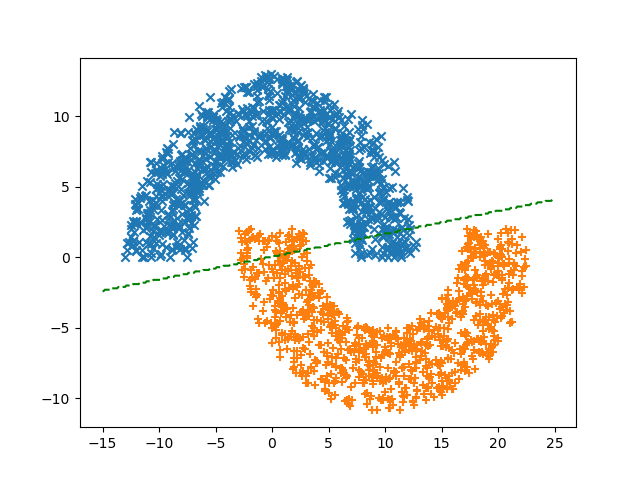
\includegraphics[scale=0.6]{code/slp.png}
	\caption{单层感知器分类结果}
\end{figure}

接着利用大作业中完成的BP神经网络训练分类模型,该模型包含两个隐藏层,下图为BP神经网络训练得到的决策边界:
\begin{figure}[H]
	\centering
	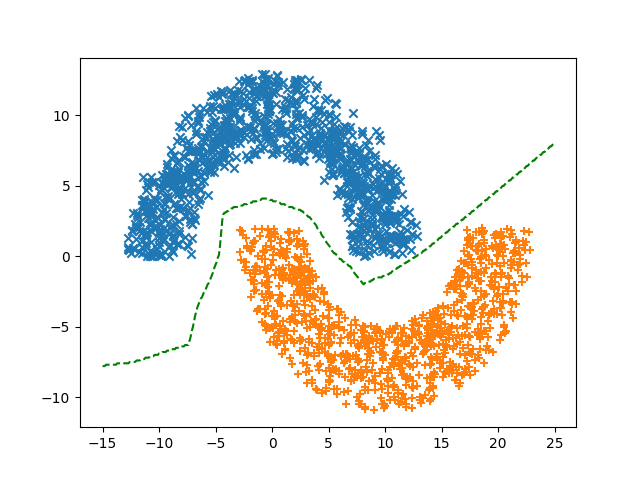
\includegraphics[scale=0.6]{code/bp.png}
	\caption{BP神经网络分类结果}
\end{figure}

综上所述,使用单层感知器无法进行非线性分类,而BP神经网络较好地完成了双月数据的分类。这是因为BP神经网络使用了隐藏层的神经元帮助学习。显而易见的,单个神经元只能学习到线性函数,而每个隐藏层神经元只需要学习决策边界中的某一段线性特征,利用隐藏层的堆叠将这些线性特征进行仿射变换从而学习到整个非线性的决策边界。

\section{}
首先下载optdigits数据集中的optdigits.tra、optdigits.tes,并从中获得训练集与测试集:
\begin{figure}[H]
	\centering
	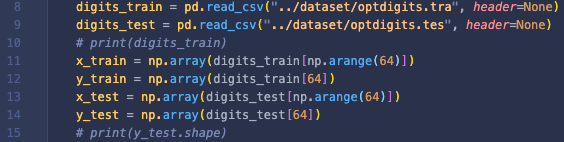
\includegraphics[scale=0.6]{dataset.png}
	\caption{optdigits数据集}
\end{figure}

调用sklearn库中的 MLPClassifier类实现单隐藏层BP网络:
\begin{figure}[H]
	\centering
	
\includegraphics[scale=0.6]{hand.png}
	\caption{MLPClassifier}
\end{figure}

通过实验求出不同神经元个数下模型最终的预测正确率:
\begin{table}[htbp]
	\centering
	\caption{\label{tab:test}神经元个数对结果影响}
	\begin{tabular}{lclcccccccc}
		\toprule    神经元 & 10 & 20& 30 & 40 & 50& 60 & 70 & 80& 90 & 100 \\
		\midrule   准确率 & 0.933 & 0.956& 0.954 & 0.958 & 0.956& 0.954 & 0.963 & 0.960& 0.962 & 0.968 \\
		\bottomrule   
	\end{tabular}  
\end{table}

通过上表绘制出神经元个数与预测准确率的关系图,由图可知随着隐藏层神经元个数的增加,预测准确率呈震荡上升趋势:
\begin{figure}[H]
	\centering
	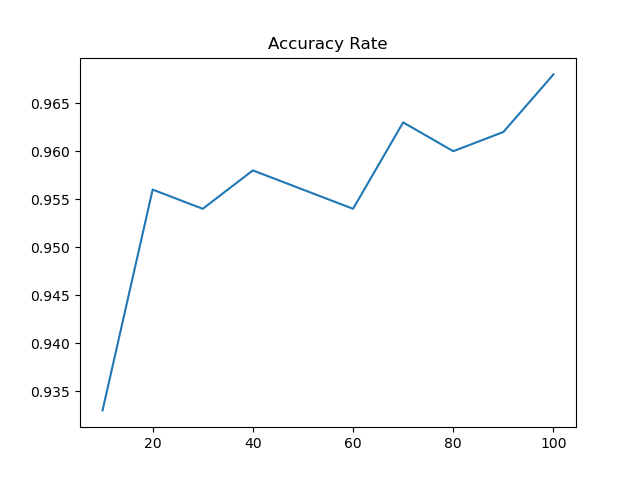
\includegraphics[scale=0.6]{code/result.png}
	\caption{神经元与准确率关系图}
\end{figure}

进一步提高预测准确率的方法:
\begin{enumerate}[1)]
	\item 增加迭代轮次;
	\item 加深模型的隐藏层;
	\item 选择不同的激活函数。
\end{enumerate}

\section{}
利用大作业一中完成的多层感知器训练规模为1-5-1的神经网络,选择均方误差作为损失函数,在完成8000轮epoch训练后,模型误差为0.01063849
\begin{figure}[H]
	\centering
	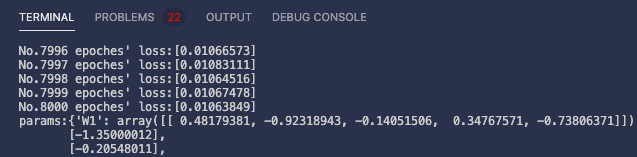
\includegraphics[scale=0.6]{loss.png}
	\caption{训练误差}
\end{figure}
由下图可知训练结果已收敛:
\begin{figure}[H]
	\centering
	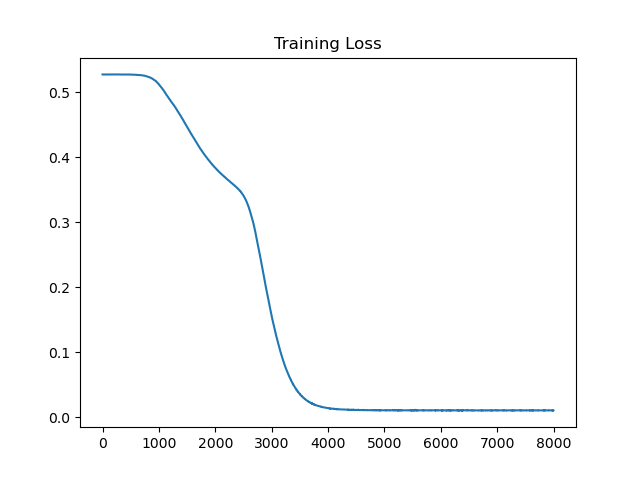
\includegraphics[scale=0.6]{code/sin_loss.png}
	\caption{sin(x)曲线损失函数}
\end{figure}
利用100个样本点训练得到的拟合结果
\begin{figure}[H]
	\centering
	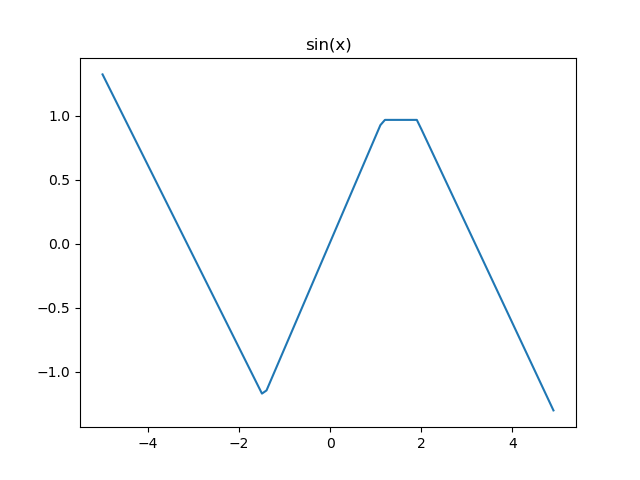
\includegraphics[scale=0.6]{code/sin.png}
	\caption{sin(x)拟合曲线}
\end{figure}

此模型隐藏层参数如下:\\

输入层-隐藏层:
\begin{equation}
	W_1=\begin{bmatrix}0.48179381\\ -0.92318943\\ -0.14051506\\  0.34767571\\ -0.73806371\end{bmatrix} \quad 	B_1=\begin{bmatrix} -0.91727367\\
	-1.35000012 \\ -0.20548011\\-0.66199873\\ 0.84841974 \end{bmatrix}
\end{equation}

隐藏层-输出层:
\begin{equation}
	W_2=\begin{bmatrix} -1.03476218\\ 1.63334207\\ 0.24860539\\-0.74677516\\-1.12417803 \end{bmatrix} \quad 	B_2=\begin{bmatrix} 0.9694142\end{bmatrix}
\end{equation}

以输入$ x=-5 $为例,计算过程为:
\begin{equation}
	y=Relu(W_1^Tx+B_1)=\begin{bmatrix} 0.04631395\\ 0 \\0 \\0.03335269\\0\end{bmatrix} \quad 	z=W_2^Ty+B_2=\begin{bmatrix} 0.89658331\end{bmatrix}
\end{equation}





\end{document}
